\section*{Результаты измерений}

С помощью метода Аббе определим фокусное расстояние тонкой линзы. Результаты вычислений фокусных расстояний для разных экспериментальных измерений представлены на рисунке:

\begin{figure}[H]
	\centering
	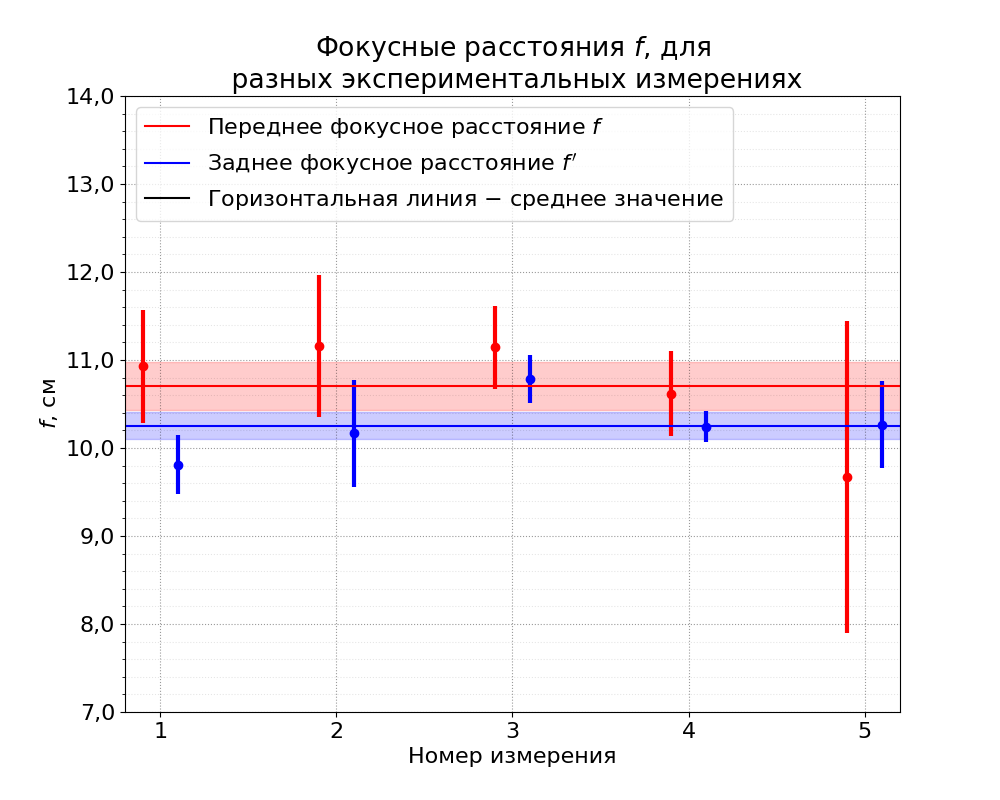
\includegraphics[width=0.88\textwidth]{../Графики/abbe_f.png}
\end{figure}

Итоговое переднее и заднее фокусные расстояния оценим как среднее:\\
Переднее фокусное расстояние $f = 10,7 \pm 0,3$ \\
Заднее фокусное расстояние $f' = 10,3 \pm 0,2$.

Случайную погрешность измерения среднего значения оценим по формуле:
$$
\sigma_{ср} = \sqrt{\frac{1}{n(n-1)} \sum\limits_{i = 1}^n (x_i - x_{ср})^2}
$$

Для тонкой линзы переднее и заднее фокусные расстояния равны. Толщину линзы оценим как разность фокусных расстояний $\delta \sim 5 \mm$. Так как $\delta$ малая величина, то итоговое фокусное расстояние оценим как среднее переднего и заднего:
$f = 10,5 \pm 0,3$.
Оптическая сила $D = 9,5 \pm 0,2 \dptr$.